% ¿Que es el aprendizaje por refuerzo?

El aprendizaje por refuerzo es una técnica de aprendizaje automático capaz de resolver problemas de forma dinámica.
Esta técnica se define como un proceso iterativo donde existe un agente capaz de tomar decisiones y un sistema dinámico influenciado por este.
Debido a la interacción entre el agente y el sistema dinámico, el agente  puede controlar el sistema a configuraciones de interés. Estas  configuraciones de interés vienen caracterizadas por una función de coste que es máxima cuando la configuración es alcanzada. 
% 
%
%Por otra parte, el aprendizaje por refuerzo y los problemas clásicos de ontrol óptimo tiene gran similitud. En los problemas de control se define un funcional de coste que depende de valor de acciones que toma el agente y del valor estado que toma el sistema a lo largo de un intervalo temporal. Sin embargo en aprendizaje por refuerzo se añade un grado de complejidad más. Mientras que en los problemas de control óptimo la relación entre las acciones y el estado del sistema es conocido para la resolución del problem, en aprendizaje por refuerzo no lo es. De esta forma, sin conocimiento del sistema el agente debe diseñar estrategicas de control solo a partir de las medidas de la acción, de l estado y de la recompensa obtenida.
%
El aprendizaje por refuerzo utiliza el principio de la programación dinámica para obtener una estrategia de actuación, sin necesidad de conocer la ecuación dinámica del sistema.
\newline

% Introducción de lo que se va a presentar
A lo largo de este capítulo describiremos formalmente el aprendizaje por refuerzo como un proceso de decisión de Markov, enseñando algunos ejemplos. 
%
Luego de esto introduciremos la programación dinámica como método para abordar el problema presentado en el marco de los procesos de decisión de Markov. 
%
Por último, mostraremos algunos algoritmos estándar para abordar este tipo de problemas.

\section{Proceso de decisión de Markov}

Un proceso de decisión de Markov es un proceso dinámico en tiempo discreto y probabilístico capaz de modelizar una gran variedad de procesos. 
%
Este marco matemático es conocido por lo menos desde la decada de 1950, donde en \cite{bellman1957theory} se escribía formalmente por primera vez.

A través de este capítulo usaremos la notación introducida en \cite[cap. 3]{sutton2018reinforcement}. 
 
\begin{defi}[Proceso de decisión de Markov]
Se define un proceso de decisión de Markov como una tupla de cuatro objetos:
\begin{itemize}
    \item Una variable aleatoria $S_t \in \Ss$, que representa el estado en la iteración $t$.
    \item Una variable aleatoria $A_t \in \As$, que representa la acción en la iteración $t$.
    \item Una variable aleatoria $R_t \in \Rs$, que representa la recompensa obtenida en la iteración $t$.
    \item Una distribución de probabilidad: 
    \begin{gather}\label{pdynamics}
        \mathbb{P}(S_{t}= s',R_{t} = r|S_{t-1} = s ,A_{t-1} = a) = p(s',r|s,a)
    \end{gather} 
    Donde a la función $p:\Ss \times \Rs \times \Ss \times \As \rightarrow [0,1]$ será llamada la \textbf{función dinámica} del proceso de decisión de Markov. Esta representa la probabilidad de que estando en el estado $s$ y tomando la acción $a$, obtengamos la recompensa $r$ y transitemos al estado $s'$. 
    \hfill\ensuremath{\square}
\end{itemize}
\end{defi}


\begin{obs}
   Aunque el espacio de recompensas puede ser infinito, a lo largo de este capítulo consideraremos que el espacio de recompensas $\Rs$ es un espacio discreto y finito. Debido a esto siempre podemos sumar en todo el espacio $\Rs$. 
\end{obs} 

Por otro lado, existe otras distribuciones de probabilidad que pueden ser obtenidas de la función dinámica $p(s',r|s,a)$. Estas distribuciones son las distribución de probabilidad de transición y de recompensa.

La distribución de probabilidad de transición $p(s'|s,a)$ se puede obtener como:

\begin{gather}\label{p(s'|s,a)}
    p(s'|s,a) =\sum_{r \in \Rs}  p(s',r|s,a)
\end{gather}

Mientras que  la distribución de probabilidad de recompensa $p(r|s,a)$ se obtiene de la siguiente manera:

\begin{gather}
    p(r|s,a) = \sum_{s' \in \Ss} p(s',r|s,a)
\end{gather}

\begin{obs}
    La distribución de probabilidad de la dinámica $p(s',r|s,a)$, la distribución de probabilidad de transición $p(s'|s,a)$ y la distribución de probabilidad de recompensa $p(r|s,a)$ son funciones distintas aunque utilicemos la misma letra $p$  para referirnos a ellas. Aunque este es un abuso de notación, podemos referirnos a las distintas distribuciones de probabilidad sabiendo que tienen número de argumentos de entrada distintos (véase el cuadro (\ref{DisNot})). 

    \begin{table}[h!]
        \centering
        \begin{tabular}{|c|c|c|}
        \hline
        \textbf{Distribución de probabilidad} &
        \textbf{Función}                      & 
        \textbf{Notación}     \\  \hline
        de la dinámica  &
        $p: \Ss \times \Rs \times \Ss \times \As \rightarrow [0,1]$ &
        $p(s'r|s,a)$ \\ \hline
        de transición   &
        $p: \Ss \times \Ss \times \As \rightarrow [0,1]$ &
        $p(s'|s,a)$ \\ \hline
        de recompensa   &
        $p: \Rs \times \Ss \times \As \rightarrow [0,1]$ &
        $p(r|s,a)$ \\ \hline        
        \end{tabular}
        \caption{Notación de distribuciones de probilidad.}
        \label{DisNot}
        \end{table}
\end{obs}
 
Por otra parte, podemos obtener la recompensa esperada debido a la acción $a$ y estando en el estado $s$ como una función $r: \Ss \times \As \rightarrow \Rs $ tal que:
\begin{gather}\label{r(s,a)}
    r(s,a) = \mathbb{E}[R_t|S_{t-1}=s,A_{t-1}=a] = 
    \sum_{s'\in\Ss} \sum_{r\in \Rs} r \ p(s',r|s,a)
\end{gather}

\begin{obs}
     La letra $r$ se utiliza para denotar  una variable aleatoria asociada a la recompensa, mientras que utilizamos la notación $r(s,a)$ para referiremos a la esperanza de la variable aleatoria $r$ debido a la acción $a$ y estando en el estado $s$. 
\end{obs}


Aunque en la definición formal de un proceso de decisión de Markov es necesario definir la distribución de probabilidad de la dinámica $p(s',r|s,a)$, es habitual definir el proceso de decisión de Markov mediante la distribución de probabilidad de transición $p(s'|s,a)$ y la distribución de probabilidad recompensa $p(r|s,a)$. 
%
Además también es posible definir un proceso de decisión de Markov, mediante la recompensa esperada $r(s,a)$ y la distribución de probabilidad de transición $p(s'|s,a)$. 
%
Estas tres formas de definir los procesos de decisión de Markov son equivalentes, sin embargo dependiendo de la aplicación una es más conveniente que otra (véase el ejemplo \ref{ControlParticula}). 



Con respecto al comportamiento del agente, se define la regla de decisión y la política para su caracterización. Estos objetos nos indican que acciones tomará el agente o como dependen estas acciones del estado.


\begin{defi}[Regla de decisión]
    En el momento de tiempo $t\in \mathbb{N}$ una \textbf{regla de decisión} es una función $\pi_t:\mathcal{S} \rightarrow \As$, que para cada elemento $s \in \mathcal{S}$ asocia $a \in \As$. 
    \hfill\ensuremath{\square}
\end{defi}

\begin{defi}[Política]
Se define como \textbf{política} de un proceso de decisión de Markov como una secuencia de reglas de decisión, $\pi = (\pi_1,\dots,\pi_T)$ que se aplican en un proceso de decisión. Podemos definir un espacio de posibles políticas $\Pi = \As\times \As \times \dots \times \As =\As^T$, tal que $\pi \in \Pi$
\hfill\ensuremath{\square}
\end{defi}

Entonces dadas esta definiciones previas podemos formular cualquier proceso de decisión de Markov. Con el objetivo ejemplificar las definiciones presentadas anteriormente veremos  un ejemplo de proceso de decisión de Markov.
 
\begin{example}[Control de una partícula]\label{ControlParticula}

    Sea el espacio de estados $\Ss = \{ s_1, s_2 ,s_3\}$  y el espacio de acciones $\As = \{\leftarrow \ , \ = \ , \ \rightarrow\}$. 
    %
    Además sea la distribución de probabilidad de transición $p(s',r|s,a)$, donde suponemos que la variable aleatoria recompensa $r$ y la variable aleatoria de estado siguiente $s'$ son independientes. 
    %
    Entonces podemos factorizar la distribución de probabilidad de la dinámica:
    \begin{gather}
        p(s',r|s,a) = p(r|s,a)p(s'|s,a)
    \end{gather}
    En este caso podemos definir la distribución $p(r|s,a)$ y la distribución $p(s'|s,a)$ por separado. Definiremos estas dos distribuciones de forma determinista. Para ello utilizaremos la función delta de Kronecker $\delta$ definida como:
    
    \begin{gather*}
        \delta(x,y) = \begin{cases}
            0 & x \neq y \\
            1 & x  = y
        \end{cases}
    \end{gather*}
    

    En primer lugar, definiremos la distribución de probabilidad de transición $p(s'|s,a)$. Para ello asociaremos cada uno de los estados $\{s_1,s_2,s_3\}$ a los vectores unitarios de $\mathbb{R}^3$: 
    \begin{gather}
        \{s_1,s_2,s_3\} \rightarrow \{(1,0,0),(0,1,0),(0,0,1)\}
    \end{gather}
    Definimos la función $f_s:\Ss \times \As \rightarrow\Ss$ como:
    \begin{gather}
        f_s(s,a) = 
        \delta(a,\leftarrow)\begin{bmatrix}
            1 & 0 & 0  \\
            1 & 0 & 0 \\
            0 & 1 & 0
        \end{bmatrix}  s + 
        \delta(a,=)\begin{bmatrix}
            1 & 0 & 0  \\
            0 & 1 & 0 \\
            0 & 0 & 1
    \end{bmatrix}  s + 
    \delta(a,\rightarrow)\begin{bmatrix}
            0 & 1 & 0  \\
            0 & 0 & 1 \\
            0 & 0 & 1
    \end{bmatrix}  s 
    \end{gather}
    Con ayuda de esta función $f_r(s,a)$ podemos definir la distribución de probabilidad $p(s'|s,a)$ como:
    
    \begin{gather}\label{deltas}
        p(s'|s,a) = \delta(s',f_s(s,a))
    \end{gather}

    En la figura (\ref{graphMDP}) se muestra un representación gráfica de la distribución de probabilidad de transición. Allí podemos ver que está definición simplemente representa una partícula que puede moverse en un recta con tres posiciones y que las acciones que podemos tomar representa un movimiento a la derecha, a la izquierda o quedarnos en la posición en la que nos encontramos. \newline

    En segundo lugar, definiremos la distribución de probabilidad de recompensa $p(r|s,a)$. Para ello definimos la función $f_r:\Ss \times \As \rightarrow \{-2,-1,9,10\}$, como:
    \begin{gather}
        f_r(s,a) = 
        \begin{cases}
            10 - \delta(a,\rightarrow) - \delta(a,\leftarrow) & s = s_2      \\
            -1 - \delta(a,\rightarrow) - \delta(a,\leftarrow) & s \neq s_2
        \end{cases}
    \end{gather}

    Entonces podemos definir la distribución de probabilidad $p(r|s,a)$ como:
    \begin{gather}\label{deltar}
        p(r|s,a) = \delta(r,f_r(s,a)) 
    \end{gather}
    
    Suponemos que el hecho de moverse penaliza en una unidad la recompensa. Además que el sistema alcanza el máximo en la posición $s=s_2$
        

    
    \begin{figure}
        \begin{subfigure}[b]{0.4\textwidth}
            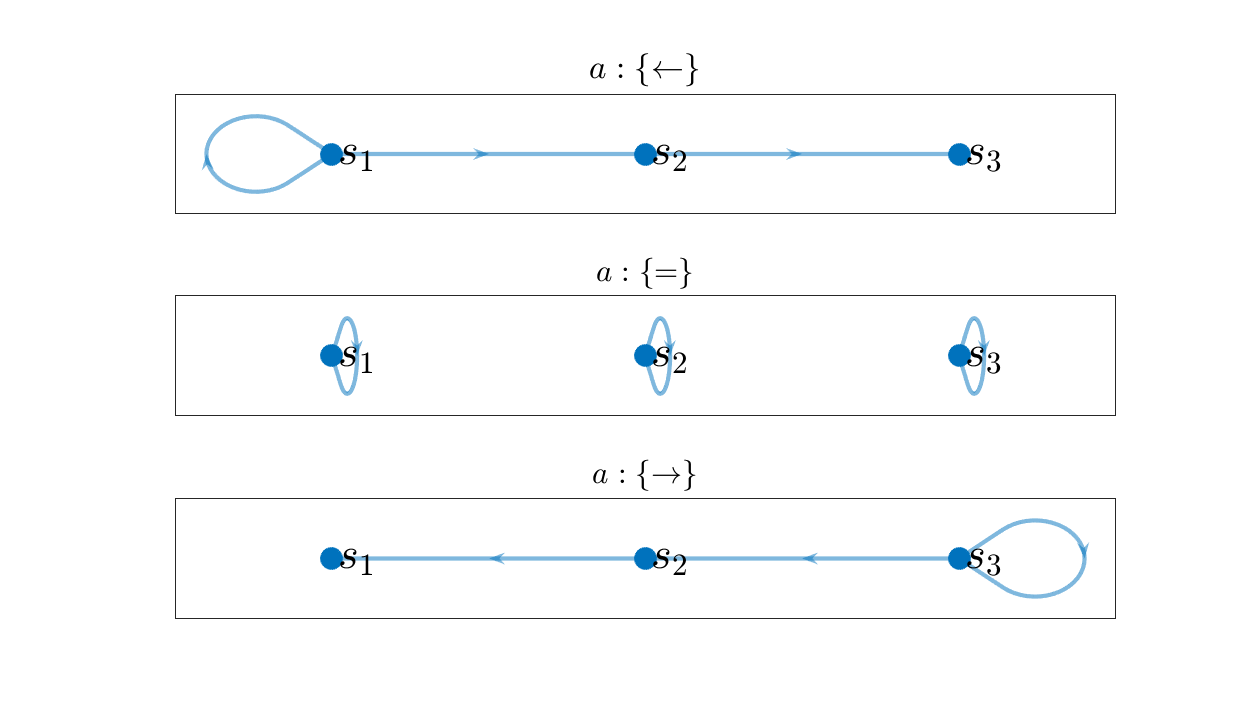
\includegraphics[scale=0.435]{img/particula_estocastica_MDP.eps}
            \caption{Proceso de decisión de Markov.}{\small Para cada posible acción se puede definir una matriz que a su vez se puede representar como un grafo.}
            \label{graphMDP}
        \end{subfigure}
        \hspace{1.75cm}
        \begin{subfigure}[b]{0.4\textwidth}
            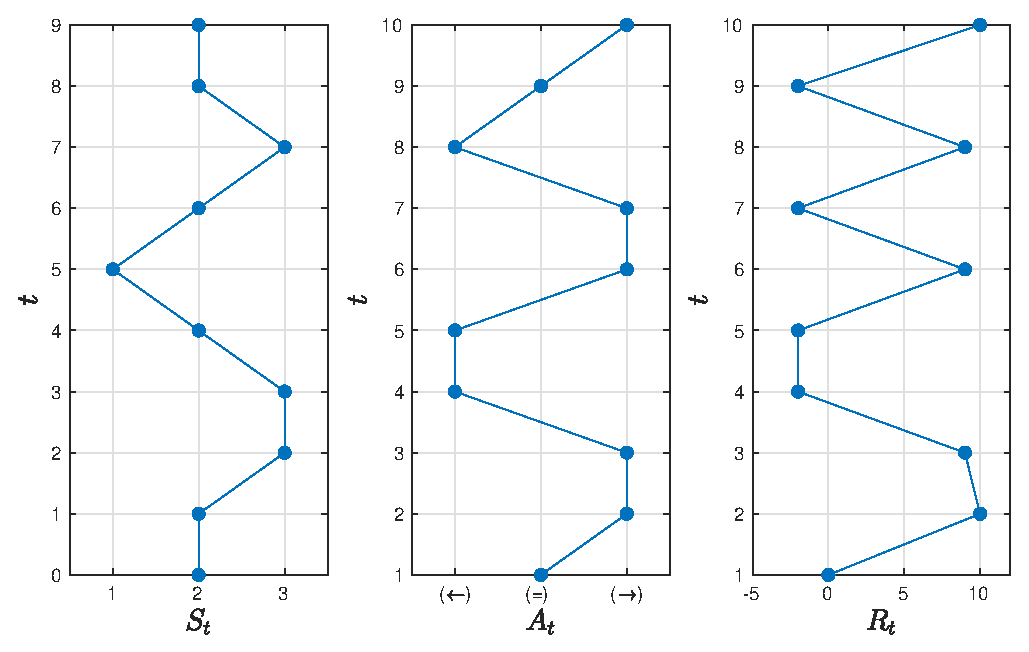
\includegraphics[scale=0.435]{img/MDP_evolution.eps}
            \caption{Evolución del sistema bajo una política.}{\small De una manera intuitiva, el agente actúa en el sistema como si tuviera un mando derecha-izquierda.}
            \label{EvolutionMDP}
        \end{subfigure}   
        \hfill
        \caption{Proceso de desición de Markov para el ejemplo (\ref{ControlParticula}) }
        \label{MDPfig}
    \end{figure}
 


    Por otra parte podemos calcular la recompensa esperada para este sistema:
    \begin{gather}
        r(s,a) = \sum_{r\in \Rs} r \sum_{s'\in\Ss} p(s',r|s,a) =         \sum_{r\in \Rs} r \sum_{s'\in\Ss} p(s'|s,a) p(r|s,a) 
    \end{gather}
    Utilizando las ecuaciones (\ref{deltar}) y(\ref{deltas}):    
    \begin{gather}
        r(s,a) = \sum_{r\in \Rs} r \sum_{s'\in\Ss} \delta(s',f_s(s,a)) \delta(r,f_r(s,a)) = f_r(s,a)  
    \end{gather}
    Asi podemos que que  $r(s,a) = f_r(s,a)$, por lo que en este ejemplo definir la distribución de probabilidad de recompensa $p(r|s,a)$ o la recompensa esperada $r(s,a)$ son equivalentes.
    
    Para concluir, notemos que con la distribución de probabilidad de transición $p(s'|s,a)$ y la distribución de probabilidad de recompensa $p(r|s,a)$, el proceso de desición de Markov del control de una partícula queda completamente caracterizado.

\end{example}

Los conceptos presentados son suficientes para definir correctamente un proceso de decisión de Markov. A partir de estos se puede definir una función de recompensa que nos determinará que tan cerca estamos a la configuración deseada. Este se llama \textbf{retorno esperado} 

\begin{defi}
Se define el \textbf{retorno esperado} a iteración $t$, como la suma de las recompensas desde la iteración $t+1$ hasta la iteración final $T$
\begin{gather}
    G_t = R_{t+1} + \gamma R_{t+2} + \gamma^2 R_{t+3} + \dots =\sum_{\tau= 0}^T \gamma^\tau R_{\tau+t+1}
\end{gather}
Donde $\gamma \in (0,1)$, es llamado el factor de descuento.
\hfill\ensuremath{\square}
\end{defi} 

\begin{obs}
    El factor de descuento $\gamma$ impide que el retorno esperado diverja cuando el horizonte temporal es $T=\infty$, siempre que las recompensas estén acotadas en todo el espacio $\Rs$. Un segundo propósito de este factor es dar más importancia las recompensas obtenidas en un tiempo cercano. 
\end{obs}
\begin{obs}[Recurencia del retorno esperado]
    Es importante notar que cuando el horizonte temporal $T$ es infinito el retorno esperado $G_t$ cumple:
    \begin{gather}\label{Gttt}
        G_t = R_{t+1} + \gamma G_{t+1}
    \end{gather}
\end{obs}

El aprendizaje por refuerzo tiene como objetivo la maximización el retorno esperado $G_t$ con respecto a la política $\pi \in \Pi$. 

\begin{problem}
    Definimos el \textbf{problema de optimización}
    \begin{gather}
              \label{eq:OCP}
            \max_{\pi \in \Pi}\mathbb{E}_\pi\bigg[ \sum_{\tau=0}^T \gamma^{\tau}R_{\tau+1} \bigg| S_0 = s \bigg] = 
            \max_{\pi \in \Pi}\mathbb{E}_\pi\big[G_0\big| S_0 = s\big]
    \end{gather}
    Donde $\mathbb{E}_\pi$ representa la esperanza con respecto a todas las posibles trayectorias en el espacio de estados tomando la política $\pi$. 
\end{problem}
La solución a este problema también tiene un carácter especial, por que lo definiremos.

\begin{defi}
    Definimos la \textbf{política óptima}, $\pi_*$ como:
    \begin{gather}
        \pi_* \in \arg \max_{\pi \in \Pi}\mathbb{E}_{\pi}\big[G_0| S_0 = s\big]  
    \end{gather}
\hfill\ensuremath{\square}
\end{defi}

Entonces un proceso de decisión de Markov en síntesis consiste maximizar el retorno esperado $G_t$ conrespecto a la  política $\pi \in \Pi$ y sujeto a la distribución de probabilidad de la dinámica $p(s',r|s,a)$.